%%%%%%%%%%%%%%%%%%%%%%%%%%%%%%%%%%%%%%%%%
% Beamer Presentation
% LaTeX Template
% Version 1.0 (10/11/12)
%
% This template has been downloaded from:
% http://www.LaTeXTemplates.com
%
% License:
% CC BY-NC-SA 3.0 (http://creativecommons.org/licenses/by-nc-sa/3.0/)
%
%%%%%%%%%%%%%%%%%%%%%%%%%%%%%%%%%%%%%%%%%

%----------------------------------------------------------------------------------------
%	PACKAGES AND THEMES
%----------------------------------------------------------------------------------------

\documentclass{beamer}

\mode<presentation> {

% The Beamer class comes with a number of default slide themes
% which change the colors and layouts of slides. Below this is a list
% of all the themes, uncomment each in turn to see what they look like.

%\usetheme{default}
%\usetheme{AnnArbor}
%\usetheme{Antibes}
%\usetheme{Bergen}
%\usetheme{Berkeley}
%\usetheme{Berlin}
%\usetheme{Boadilla}
%\usetheme{CambridgeUS}
%\usetheme{Copenhagen}
\usetheme{Darmstadt}
%\usetheme{Dresden}
%\usetheme{Frankfurt}
%\usetheme{Goettingen}
%\usetheme{Hannover}
%\usetheme{Ilmenau}
%\usetheme{JuanLesPins}
%\usetheme{Luebeck}
%\usetheme{Madrid}
%*\usetheme{Malmoe}
%\usetheme{Marburg}
%\usetheme{Montpellier}
%\usetheme{PaloAlto}
%\usetheme{Pittsburgh}
%\usetheme{Rochester}
%\usetheme{Singapore}
%\usetheme{Szeged}
%\usetheme{Warsaw}

% As well as themes, the Beamer class has a number of color themes
% for any slide theme. Uncomment each of these in turn to see how it
% changes the colors of your current slide theme.

%\usecolortheme{albatross}
%\usecolortheme{beaver}
%\usecolortheme{beetle}
%\usecolortheme{crane}
%\usecolortheme{dolphin}
%\usecolortheme{dove}
%\usecolortheme{fly}
%\usecolortheme{lily}
\usecolortheme{orchid}
%\usecolortheme{rose}
%\usecolortheme{seagull}
%\usecolortheme{seahorse}
%\usecolortheme{whale}
%\usecolortheme{wolverine}

%\setbeamertemplate{footline} % To remove the footer line in all slides uncomment this line
%\setbeamertemplate{footline}[page number] % To replace the footer line in all slides with a simple slide count uncomment this line

%\setbeamertemplate{navigation symbols}{} % To remove the navigation symbols from the bottom of all slides uncomment this line
}


\usepackage{graphicx} % Allows including images
\usepackage{booktabs} % Allows the use of \toprule, \midrule and \bottomrule in tables
\usepackage{xspace}
\usepackage{caption}
\usepackage{subfigure}
\usepackage[english,brazil]{babel}
\usepackage[utf8]{inputenc}

%Renomeia o nome padrao das figuras.
\renewcommand{\figurename}{Figura}
\renewcommand{\tablename}{Tabela}



\usepackage[pygopt={texcomments=true,style=emacs}]{pythontex}
\setpythontexlistingenv{listing}

\newcounter{sublisting}[listing]
\newcommand{\codeline}[1]{%
  \addcontentsline{lopytx}{listing}%
    {\protect\numberline{\hspace{0.5in}\thelisting.\arabic{FancyVerbLine}}\hspace{0.5in}#1}%
}


%----------------------------------------------------------------------------------------
%	TITLE PAGE
%----------------------------------------------------------------------------------------

\title[Computação Gráfica]{Preenchimento de Polígonos} % The short title appears at the bottom of every slide, the full title is only on the title page

\author{Uéliton Freitas} % Your name
\institute[UFMS] % Your institution as it will appear on the bottom of every slide, may be shorthand to save space
{
Universidade Católica Dom Bosco - UCDB \\ % Your institution for the title page
\medskip
\textit{freitas.ueliton@gmail.com} % Your email address
}
\date{\today} % Date, can be changed to a custom date


\begin{document}

\begin{frame}
\titlepage % Print the title page as the first slide
\end{frame}

\begin{frame}
\frametitle{Sumário} % Table of contents slide, comment this block out to remove it
\tableofcontents % Throughout your presentation, if you choose to use \section{} and \subsection{} commands, these will automatically be printed on this slide as an overview of your presentation
\end{frame}




%----------------------------------------------------------------------------------------
%	PRESENTATION SLIDES
%----------------------------------------------------------------------------------------

%------------------------------------------------
\section{Introdução} 
%------------------------------------------------

%\section{Speeded-Up Robust Features - SURF} % A subsection can be created just before a set of slides with a common theme to further break down your presentation into chunks
%\section{Baf Of Features and Colors}

%\section{Refer\^encias}
%%%%%%%%%%%%%%%%%%%%%%%%%%%%%%%%%%%%%%%%%%%%%%%%%%%%%%%%%%%%%%%%%%%%%%%%%%%%%%%%%%%%%%%%%%
\begin{frame}
\frametitle{Introdução}

		\begin{block}{Preenchimento de Polígonos}
		\begin{itemize}
			\item Além do desenho de linhas, uma outra construção útil é o \textbf{preenchimento de áreas}.
				\begin{itemize}
					\item Usado para descrever superfícies ou objetos sólidos.
				\end{itemize}
			\item Embora qualquer forma possa ser preenchida, normalmente as \textbf{APIs gráficas suportam polígonos}.
				\begin{itemize}
					\item Maior eficiência por serem descritos por equações lineares.
					\item Maioria das superfícies curvas podem ser aproximadas por polígonos. 
				\end{itemize}
		\end{itemize}
		\end{block}
	
\end{frame}

%%%%%%%%%%%%%%%%%%%%%%%%%%%%%%%%%%%%%%%%%%%%%%%%%%%%%%%%%%%%%%%%%%%%%%%%%%%%%%%%%%%%%%%%%%
\begin{frame}
\frametitle{Introdução}

		\begin{block}{Preenchimento de Polígonos}
		\begin{itemize}
			\item Aproximação de curva é normalmente chamada de \textbf{tesselação} de uma superfície ou \textbf{malha de polígonos}.
				\item Estas aproximações podem ser rapidamente geradas como visões wire-frame.
		\end{itemize}
		\end{block}
		
		\begin{figure}[!h]
			\begin{center}
				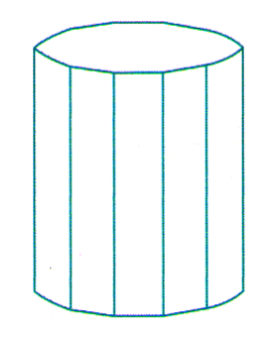
\includegraphics[width=0.3\textwidth]{Figures/WirFra}
			\end{center}
		\end{figure}
	
\end{frame}

%%%%%%%%%%%%%%%%%%%%%%%%%%%%%%%%%%%%%%%%%%%%%%%%%%%%%%%%%%%%%%%%%%%%%%%%%%%%%%%%%%%%%%%%%%
\begin{frame}
\frametitle{Introdução}

		\begin{block}{Preenchimento de Polígonos}
		\begin{itemize}
			\item Um polígono é uma \textbf{figura plana} especificada por um conjunto de 3 ou mais \textbf{vértices}, \textbf{ligados} sequencialmente por \textbf{arestas}(linhas).
			\item Arestas possuem pontos em comum somente em seu ponto inicial e final.
			\item Todos os vértices estão no mesmo plano.
			\item Devido a erros de arredondamento, as arestas de um polígono podem são ser coplanares.
			\begin{itemize}
				\item Utiliza-se triângulos para resolver este problema.
			\end{itemize}
		\end{itemize}
		\end{block}
	
\end{frame}

%%%%%%%%%%%%%%%%%%%%%%%%%%%%%%%%%%%%%%%%%%%%%%%%%%%%%%%%%%%%%%%%%%%%%%%%%%%%%%%%%%%%%%%%%%
\begin{frame}
\frametitle{Introdução}

		\begin{block}{Classificação de Polígonos}
		\begin{itemize}
			\item Se todos os ângulos interiores de um polígono forem menores que $180^\circ$, o polígono é \textbf{convexo} caso contrário é \textbf{côncavo}.
				\item Em um polígono convexo, dois pontos interiores definem um segmento de reta também no interior.
		\end{itemize}
		\end{block}
		
		\begin{figure}[!h]
			\begin{center}
				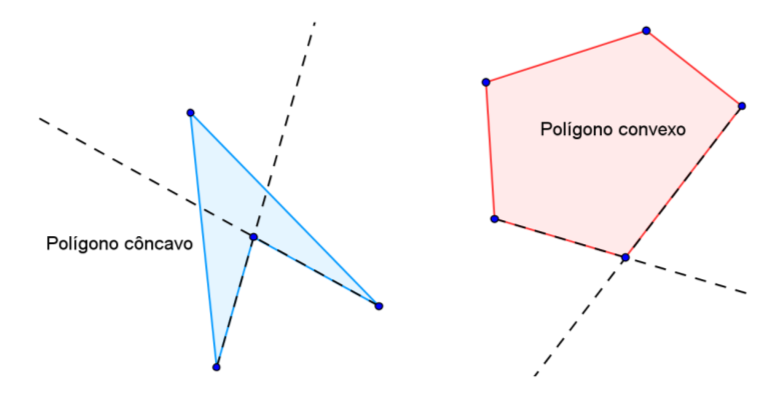
\includegraphics[width=0.6\textwidth]{Figures/Pol}
			\end{center}
		\end{figure}
	
\end{frame}

%%%%%%%%%%%%%%%%%%%%%%%%%%%%%%%%%%%%%%%%%%%%%%%%%%%%%%%%%%%%%%%%%%%%%%%%%%%%%%%%%%%%%%%%%%
\begin{frame}
\frametitle{Introdução}

		\begin{block}{Classificação de Polígonos}
		\begin{itemize}
			\item O termo polígono \textbf{degenerado} descreve um polígono com vértices colineares, ou que apresentam vértices repetidos.
			\item Uma \textbf{API} gráfica para ser \textbf{robusta} deve \textbf{regeitar} polígonos \textbf{não planares ou degenerados}.
			\begin{itemize}
				\item Na verdade isso é deixado a cargo do programador.
			\end{itemize}
		\end{itemize}
		\end{block}
		
		\begin{figure}[!h]
			\begin{center}
				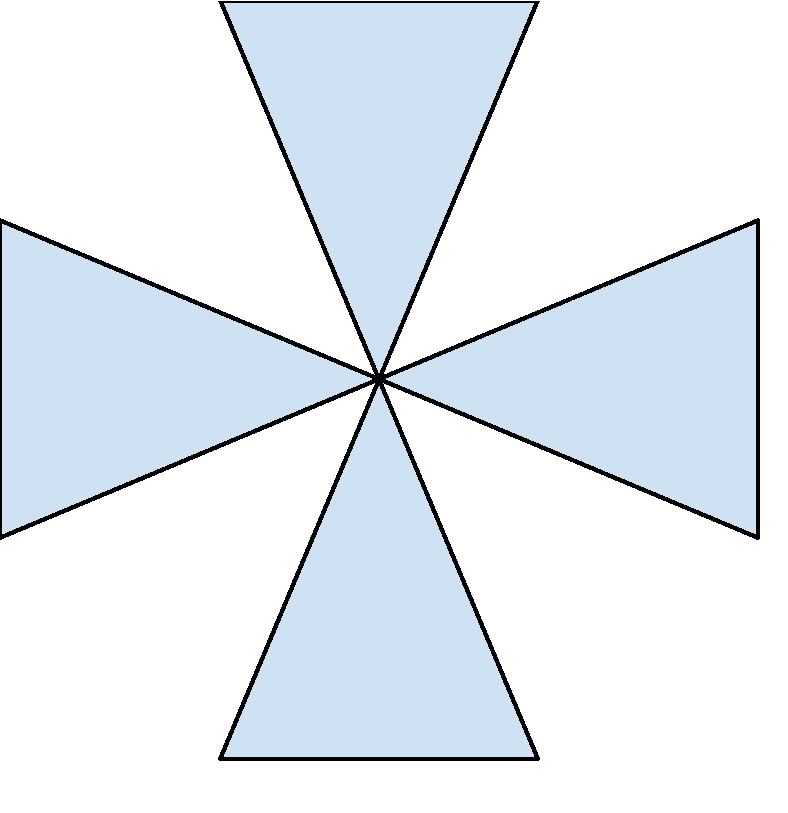
\includegraphics[width=0.3\textwidth]{Figures/PolDeg}
			\end{center}
		\end{figure}
	
\end{frame}

%%%%%%%%%%%%%%%%%%%%%%%%%%%%%%%%%%%%%%%%%%%%%%%%%%%%%%%%%%%%%%%%%%%%%%%%%%%%%%%%%%%%%%%%%%
\begin{frame}
\frametitle{Introdução}

		\begin{block}{Classificação de Polígonos}
		\begin{itemize}
			\item \textbf{APIs} gráficas trabalham apenas com com \textbf{polígonos convexos}.
			\begin{itemize}
				\item Melhor dividir um polígono côncavo em um conjunto de polígonos convexos.
				\item \textbf{OpenGL} requer que todos os polígonos sejam convexos.
			\end{itemize}
		\end{itemize}
		\end{block}
		
		\begin{figure}[!h]
			\begin{center}
				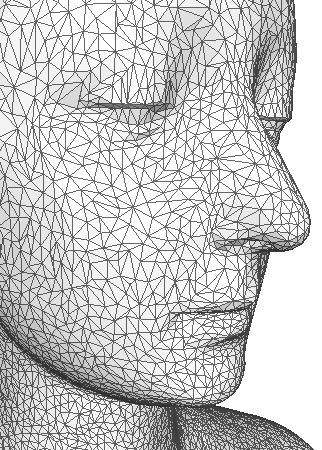
\includegraphics[width=0.25\textwidth]{Figures/TriMes}
			\end{center}
		\end{figure}
	
\end{frame}

%%%%%%%%%%%%%%%%%%%%%%%%%%%%%%%%%%%%%%%%%%%%%%%%%%%%%%%%%%%%%%%%%%%%%%%%%%%%%%%%%%%%%%%%%%
\begin{frame}
\frametitle{Introdução}

		\begin{block}{Identificando Polígonos Côncavos}
		\begin{itemize}
			\item Cria-se vetores com as arestas e faz-se  o produto vetorial sobre arestas adjacentes.
				\begin{itemize}
					\item A \textbf{coordenada-z} de todos os produtos \textbf{devem ter o mesmo sinal} em um polígono \textbf{convexo}.
				\end{itemize}
		\end{itemize}
		\end{block}
		
		\begin{figure}[!h]
			\begin{center}
				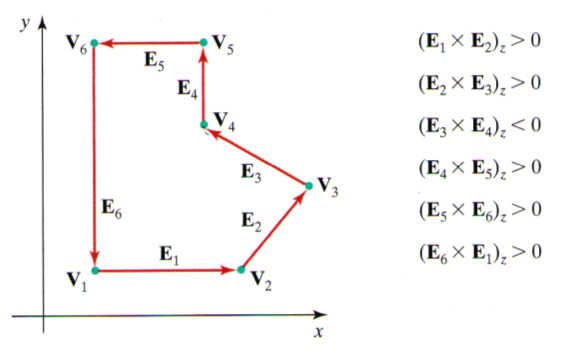
\includegraphics[width=0.5\textwidth]{Figures/PolConAre}
			\end{center}
		\end{figure}
	
\end{frame}


%%%%%%%%%%%%%%%%%%%%%%%%%%%%%%%%%%%%%%%%%%%%%%%%%%%%%%%%%%%%%%%%%%%%%%%%%%%%%%%%%%%%%%%%%%
\begin{frame}
\frametitle{Introdução}

		\begin{block}{Dividindo Polígonos Côncavos}
		\begin{itemize}
			\item Cria-se vetores para dois vértices consecutivos.
				\begin{itemize}
					\item $E_k = V_{k+1} - V_k$
				\end{itemize}
			\item Calcular o produto vetorial destes no sentido anti-horário.
			\item Se algum produto for negativo, o polígono é côncavo
				\begin{itemize}
					\item Dividindo o polígono ao longo da linha do primeiro vértice.
				\end{itemize}
		\end{itemize}
		\end{block}
		
		\begin{figure}[!h]
			\begin{center}
				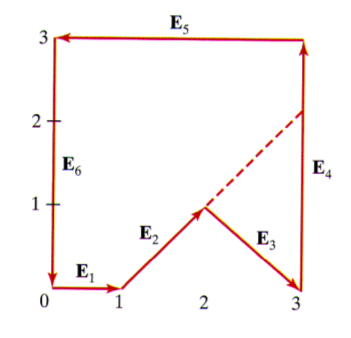
\includegraphics[width=0.35\textwidth]{Figures/PolConVexDiv}
			\end{center}
		\end{figure}
	
\end{frame}

%----------------------------------------------------------------------------------------
\end{document} 